\chapter[\hspace{0pt}模型建立与求解]{{\heiti\zihao{3}\hspace{0pt}模型建立与求解}}\label{chapter4: 模型建立与求解}
% \setcounter{page}{4} % 这里要在论文摘要和符号表写完后手动修改页码

\removelofgap
\removelotgap

%% 文章标题架构
% 一级 chapter      : \chapter[\hspace{0pt}模型建立与求解]{{\heiti\zihao{3}\hspace{0pt}模型建立与求解}}\label{chapter4: 模型建立与求解}
% 二级 section      : \section[\hspace{-2pt}问题1:路旅游方案设计]{{\heiti\zihao{-3} \hspace{-8pt}问题1:路旅游方案设计}}\label{section3: 问题1:路旅游方案设计}
% 三级 subsection   : \subsection[\hspace{-2pt}模型建立与求解]{{\heiti\zihao{4} \hspace{-8pt}模型建立与求解}}\label{section3: 模型建立与求解}
% 四级(顶格)        : \noindent\textbf{(1)参数编码与搜索空间}
% 四级(不顶格)      : \textbf{}
% 五级(尽量别用)    : \circled{1} \textbf{$\Delta E_{00}$损失值统计}
% 
%% 公式、图片、表格

% 公式:
% 1. 中间不必加上$$符号
% 2. 在equation后面加上*可以不要自动编号
% \begin{equation}
% \begin{aligned}
%   &u_{i,j}=
%   \begin{cases}
%     v_{i,j}^{(t)},&\text{if } \mathrm{rand}_j\le CR\text{ or } j=j_{rand},\\
%     x_{i,j}^{(t)},&\text{otherwise},
%   \end{cases}
% \end{aligned}
% \end{equation}

% 图片:
% \begin{figure}[h]
% \centering
% \captionsetup{font={small, stretch=1.312}}
% 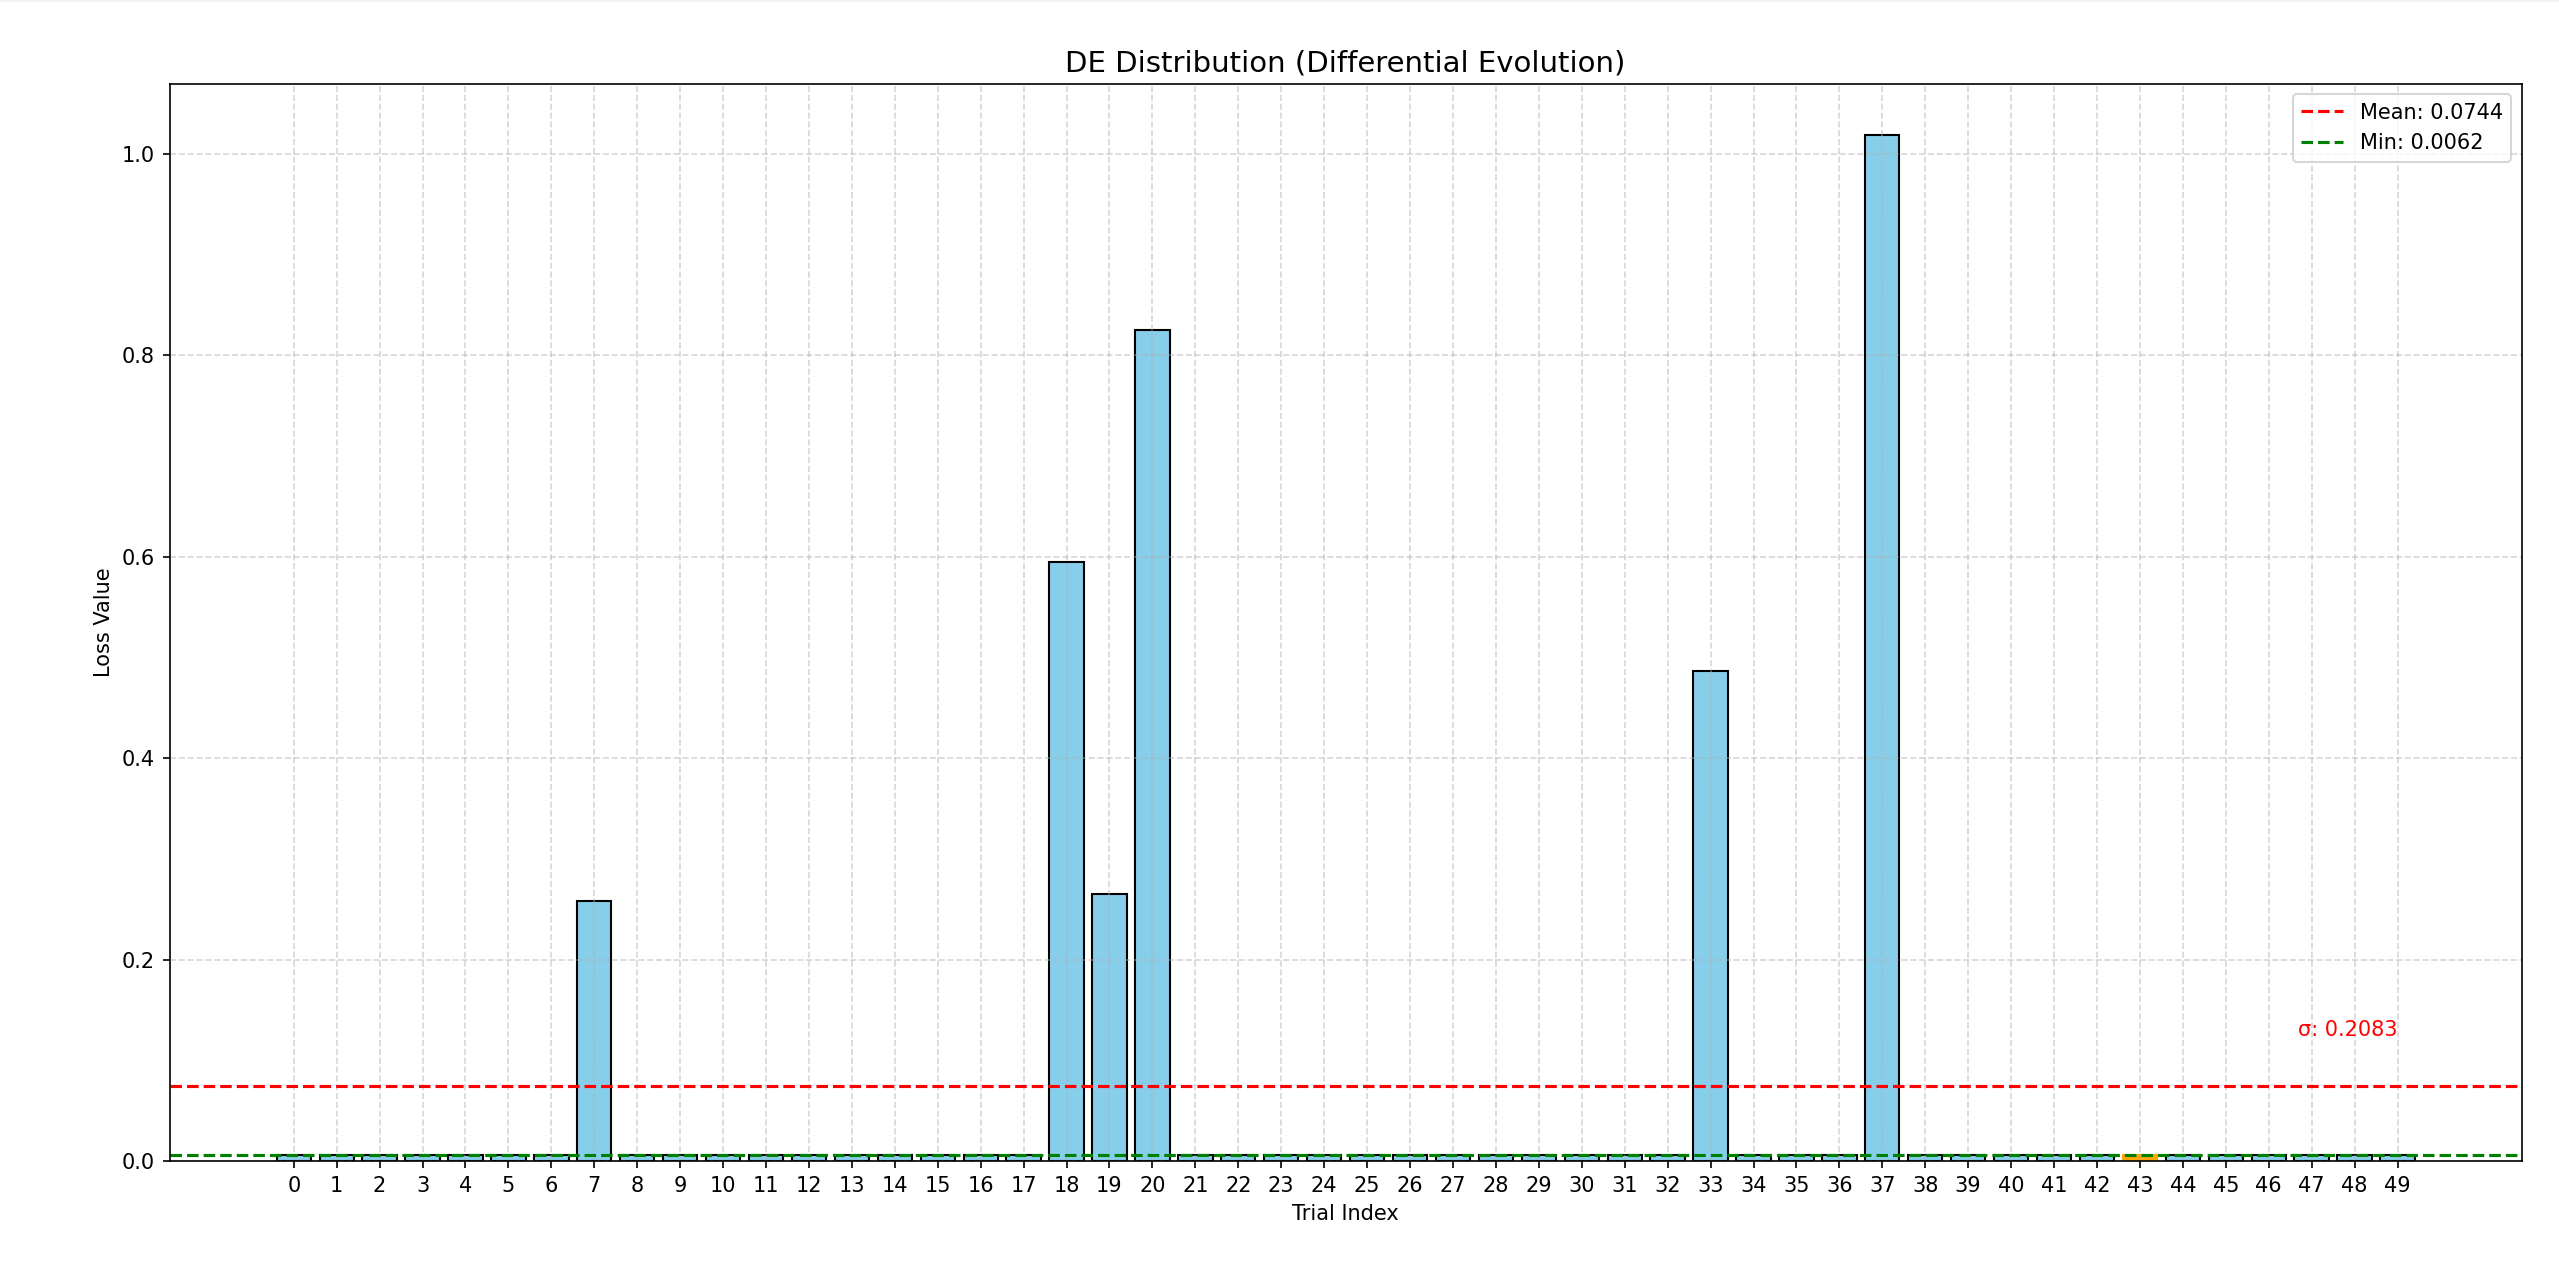
\includegraphics[width=1.0\columnwidth]{figures/DE2000.png}
% \bicaption[50次独立优化实验柱状损失图]{50次独立优化实验柱状损失图。}[Histogram of loss values from 50 independent optimization experiments]{Histogram of loss values from 50 independent optimization experiments.}
% \label{figure3: 柱状loss}
% \end{figure}
% 引用方式:在文字后面加上:\ref{figure3: 柱状loss}

% 表格:
% \begin{table}[h!]
% \small    % 设置表格字体为5号
% \setstretch{1.245}        % 设置具有指定弹力的橡皮长度(原行宽的1.2倍)
% \captionsetup{font={small, stretch=1.512}}
% \centering
%\bicaption[不同基色图像的伽马参数估计结果]{不同基色图像的伽马参数估计结果。}[Gamma parameter estimation results for different primary color images]{Gamma parameter estimation results for different primary color images.}    % 中英文标题


\section[\hspace{-2pt}问题一:路旅游方案设计]{{\heiti\zihao{-3} \hspace{-8pt}问题一:路旅游方案设计}}\label{section3: 问题1:路旅游方案设计}

\subsection[\hspace{-2pt}模型建立与求解]{{\heiti\zihao{4} \hspace{-8pt}模型建立与求解}}\label{section3: 模型建立与求解}

对于此问题,我们首先通过Floyd‑Warshall算法补全邻接矩阵,得到任意两点之间的最短距离。这样我们就可以得到任意区域到任意景点的交通费用和交通时间。此外,我们还需要考虑到旅游信息(住宿、美食、景点等)对方案的影响。既要考虑其对方案满意度的增益,也应当考虑到可容纳人数的限制。\cite{ZNXT201901008}以此为基础,我们进行以下建模:

\textbf{景点收益:}由于缺乏具体景点评分数据,我们假设每个景点具有相近的吸引力价值,即此处不加入游客对景点的偏好因素。$P_{max}$表示某一类型的方案的最大满意度(即总是选择游客喜好程度最高的区域3)。

\begin{equation}
  \begin{aligned}
  \text{Pref}^{(d_{p})}_{max}(type)=\begin{cases}
  9\times 1+2=11, & \text{(1日)}\\
  9\times 3+4=31, & \text{(2日)}\\
  9\times 5+6=51, & \text{(3日)}
  \end{cases}
  \end{aligned}
  \end{equation}

以上方程为景区最大收益函数。为了减少数值对模型计算的影响,我们对三种收益进行归一化处理。

\textbf{区域收益:}套餐$p$涉及到的区域的用餐以及住宿体验。根据题目数据,我们将区域喜好度评分$P_{R_{j}}$作为游客在该区域用餐/住宿获得的满意度。如果套餐跨多日,可能涉及多个不同的区域,则将相应区域的偏好分累计。若在同一天中午和晚上都在同一$R_{j}$区域,则游客在该天对区域$R_{j}$的体验包括午餐和晚餐+住宿,为方便建模并突出问题的重心,我们采用叠加的方式计算区域满意度。

\textbf{交通的时间与费用成本:}每套旅游方案中的交通费用和时间开销会降低满意度。我们采用函数$Cost(p)$来评价一个方案中的所有交通费用,用$Time(p)$来表示所有时间开销。此外我们为其增加了权重$w_{\text{cost}}, w_{\text{time}}$,以此代表不同套餐的倾向,用以区分经济优先还是时间优先。

\begin{equation}
\begin{aligned}
  \text{Cost}(p) = \sum_{(S_i,R_j)\in p}{d(S_i,R_j)}
\end{aligned}
\end{equation}

\begin{equation}
  \begin{aligned}
    \text{Time}(p) = \sum_{(S_i,R_j)\in p}{t(S_i,R_j)}
  \end{aligned}
\end{equation}
  



总的某方案$p$的满意度函数如下:

\begin{equation}
\begin{aligned}
  u_p \;=\; w_{\text{pref}}\frac{\text{Pref}(p)}{\text{Pref}_{\max}^{(d_p)}} \;-\; w_{\text{cost}}\frac{\text{Cost}(p)}{\max\{\text{Cost}(q):q\in \mathcal{P}\}} \;-\; w_{\text{time}}\frac{\text{Time}(p)}{\max\{\text{Time}(q):q\in \mathcal{P}\}},
\end{aligned}
\end{equation}

\textbf{最大化函数:}
\begin{equation}
  \begin{aligned}
    Z = \sum_{p\in \mathcal{P}}u_{p}\cdot x_{p}.
  \end{aligned}
\end{equation}

约束条件如下:

\noindent\textbf{1.景点接待容量限制:}
各景点在各个半天时段的接待总人数不得超限。由于早午两段和最多3天行程共有6个半天时段,模型将假设景点容量可在不同时段重复利用。对每个景点 $i\in S$ 有:

\begin{equation}
  \begin{aligned}
    \sum_{p\in \mathcal{P}}\delta_{i,p}\cdot x_{p} \leq 6\,C_{S_{i}},\quad i=1,2\dots ,6,
  \end{aligned}
\end{equation}
其中$\delta_{i,p}=1$当路线$p$包含景点$i$(即游客在某一时段游览了景点$i$),否则$\delta_{i,p}=0$。

\noindent\textbf{2.午餐餐厅容量约束:}
每个区域的午餐接待能力(每天中午)也限制了路线分配。类似地,如果认为最多3个中午时段可复用,则对每个区域 $j\in R$:

\begin{equation}
  \begin{aligned}
    \sum_{p\in \mathcal{P}}\theta_{j,p}\cdot x_{p} \leq 3\,L_{R_{j}},\quad j=1,2,\dots ,6,
  \end{aligned}
\end{equation}
其中$theta_{j,p}$代表路线$p$在中午曾安排于区域$j$就餐次数(一日游有1次午餐、三日游有3次午餐机会,但可能某些路线会重复去某一区域)。代码中简化为每个区域午餐总游客$\le C^{\text{lunch}}_j$,相当假定所有行程共用一个中午时段容量,这在行程跨多日的情况下略趋保守。

\noindent\textbf{3.晚餐及住宿容量约束:}
每个区域用于晚餐和住宿的容量在不同夜晚也可重复利用。三日游行程最多涉及2晚,故每区域最多2个夜晚可安排住宿。对每个区域 $j\in R$:
\begin{equation}
  \begin{aligned}
    \sum_{p\in \mathcal{P}}\phi_{j,p}\cdot x_p \;\le\; 2\,C^{\text{night}}_j, \quad j=1,\dots,6,
  \end{aligned}
\end{equation}

其中$\phi_{j,p}$为路线$p$在夜晚留宿于区域$j$的次数(二日游路线有1晚、三日游有2晚,一般假定同一线路不重复入住同一酒店区域)。

\noindent\textbf{4.游客总数约束:}
根据预期需求,分别规定各类行程分配的总游客数。例如,设定选择一日游的游客总数为$N_{1}$人、二日游$N_{2}$人、三日游$N_{3}$人。则对每一种行程类型分别有:
\begin{equation}
  \begin{aligned}
    \sum_{p\in P_{1\text{day}}}x_p = N_{1},\qquad \sum_{p\in P_{2\text{day}}}x_p = N_{2},\qquad \sum_{p\in P_{3\text{day}}}x_p = N_{3}.    
  \end{aligned}
\end{equation}

代码实现中分别令一日游、二日游总游客数为30,000,三日游为20,000。

约束处理完成后,我们将采用枚举的方式得到一日游、二日游等的所有可能方案。再将其加入到MILP模型中。结合遗传算法选择高质量路线,并采用启发式规则进行路线多样化拓展。最终得到最合适的旅游路线。

\subsection[\hspace{-2pt}问题一结果分析]{{\heiti\zihao{4} \hspace{-8pt}问题一结果分析}}\label{section4: 问题一结果分析}

根据$w_{cost}$和$w_{time}$的不同权重配置,我们可以设置不同权重,得到不同侧重点的旅游方案。本论文设置了三种情况,并对优化结果进行了详细分析。

\textbf{均衡型(费用权重=0.5,时间权重=0.5):}

均衡型配置追求费用和时间的平衡优化。实验结果显示:一日游方案成功分配3万游客到2条最优路线,平均满意度达到0.47;二日游方案分配3万游客到4条路线,总费用302.7万元,总时间5541万分钟,平均满意度0.39;三日游方案分配2万游客到4条路线,总费用355.06万元,平均满意度0.34。该配置在各项指标间取得了良好的平衡,适合大多数游客的需求。

\textbf{费用优先型(费用权重=0.7,时间权重=0.3):}

费用优先型配置更注重控制旅游成本。对比分析发现:在一日游方案中,费用优先型与均衡型结果完全一致,说明一日游路线已达到成本最优;二日游方案中,总费用降低至292.92万元,相比均衡型节省了9.78万元(降幅3.2%),但时间成本略有增加至5745万分钟;三日游方案表现最为突出,总费用大幅降低至341.32万元,相比均衡型节省13.74万元(降幅3.9%),同时平均满意度还提升至0.36。这表明费用优先型配置能够有效控制成本,特别适合预算敏感的游客群体。

\textbf{时间优先型(费用权重=0.3,时间权重=0.7):}

时间优先型配置侧重于减少旅行时间。结果显示:一日游和二日游方案与均衡型完全相同,表明在这两种方案中时间已达到最优配置;三日游方案中,虽然总费用略有增加至367.6万元,但时间安排更为紧凑高效。值得注意的是,时间优先型在路线选择上呈现出不同的偏好模式,优先选择时间效率更高的景点组合和区域路径,适合时间有限但希望充分体验的游客。

\textbf{综合比较分析:}

通过三种配置的对比分析可以发现:(1)一日游方案在三种配置下结果一致,说明短期旅游路线的优化空间有限,已达到全局最优;(2)二日游方案中费用优先型在成本控制方面具有明显优势,适合预算约束较强的情况;(3)三日游方案显示出最大的优化弹性,不同权重配置产生显著差异,为不同需求的游客提供了多样化选择;(4)所有配置均成功实现了大规模游客分流,验证了模型的实用性和有效性。这些结果为旅游管理部门制定差异化的旅游产品策略提供了科学依据。



\section[\hspace{-2pt}问题二:方案优化]{{\heiti\zihao{-3} \hspace{-8pt}问题二:方案优化}}\label{section3: 问题2:方案优化}

\subsection[\hspace{-2pt}问题分析与建模目标]{{\heiti\zihao{4} \hspace{-8pt}问题分析与建模目标}}\label{section2: 问题分析与建模目标}

根据问题分析,我们设计了如下的距离函数,综合考虑了方案间的景点、路线、区域等相似度,将重复性较强的方案合并。由于景点和区域皆为符号度量,因此二者都采用了Jaccard相似度。类型相似度用以判断旅游天数是否相同,可以保证同一聚类中心皆为同一天数。余下的偏好相似度、成本相似度和时间相似度都采用了欧氏距离,成本相似度采用了欧氏距离,时间相似度采用了欧氏距离。

\noindent\textbf{1.景点相似度:}
\begin{equation}
  \begin{aligned}
    \text{Simu}_{p_{i},p_{j},S} = \frac{|\underset{S\in p_i}{\bigcup}\cap \underset{S\in p_j}{\bigcup}|}{|\underset{S\in p_i}{\bigcup}\cup \underset{S\in p_j}{\bigcup}|}
  \end{aligned}
\end{equation}

\noindent\textbf{2.类型相似度:}
\begin{equation}
  \begin{aligned}
    \text{Simu}_{p_{i},p_{j},Day} = \begin{cases}
      1, & \text{若}d_{p_i}=d_{p_j}\\
      0, & \text{否则}
    \end{cases}
  \end{aligned}
\end{equation}

\noindent\textbf{3.区域相似度:}
\begin{equation}
  \begin{aligned}
    \text{Simu}_{p_{i},p_{j},R} = \frac{|\underset{R\in p_i}{\bigcup}\cap \underset{R\in p_j}{\bigcup}|}{|\underset{R\in p_i}{\bigcup}\cup \underset{R\in p_j}{\bigcup}|}
  \end{aligned}
\end{equation}

\noindent\textbf{4.偏好相似度:}
\begin{equation}
  \begin{aligned}
    \text{Simu}_{p_{i},p_{j},P} = 1-\frac{|\text{Pref}(p_{i})-\text{Pref}(p_{j})|}{\text{max}(\text{Pref}(p_{i}),\text{Pref}(p_{j}))}
  \end{aligned}
\end{equation}

\noindent\textbf{5.成本相似度:}
\begin{equation}
  \begin{aligned}
    \text{Simu}_{p_{i},p_{j},C} = 1-\frac{|\text{Cost}(p_{i})-\text{Cost}(p_{j})|}{\text{max}(\text{Cost}(p_{i}),\text{Cost}(p_{j}))}
  \end{aligned}
\end{equation}

\noindent\textbf{6.时间相似度:}
\begin{equation}
  \begin{aligned}
    \text{Simu}_{p_{i},p_{j},T} = 1-\frac{|\text{Time}(p_{i})-\text{Time}(p_{j})|}{\text{max}(\text{Time}(p_{i}),\text{Time}(p_{j}))}
  \end{aligned}
\end{equation}

定义好以上相似度后,就可以计算两个方案之间的加权距离。

\begin{equation}
  \begin{aligned}
    D(p_{i},p_{j}) = \sum_{k\in \text{Temp}}^{6}w_{k}\cdot\text{Simu}_{p_{i},p_{j},k},\quad \text{Temp}=\{S,Day,R,P,C,T\}
  \end{aligned}
\end{equation}

以上因素综合考虑到不同旅行方案在景点、区域、偏好等多个方面的相似度,可以得到不同旅行方案之间的距离。在完成“旅游方案相似度”加权距离函数的数学建模后,下一步便可对所有候选路线实施 K‑means 聚类。

% 基于旅游方案相似度的加权距离函数建模完成后,即可进行K均值聚类。算法会尝试不同的K值,并根据簇内平方和选择最优的K值作为最终的结果。

% 当要求旅游套餐种类总数不超过10种时,需要对上述模型进行适应性修改。原模型在追求最大满意度下,可能启用许多不同路线方案来绕开局部容量瓶颈,从而方案种类较多。如果限制套餐类型数$\le10$,模型必须在满意度与管理简化之间折中。我们做出了如下调整:

% \noindent\textbf{加入套餐数量约束:}增加约束$\displaystyle\sum_{p\in P} \le 10$,限制被选用的不同路线方案数不超过10种。其中为0-1变量,表示方案$p$是否被采用。并引入逻辑约束$x_p \le N_{\text{total}};$(或大$M$法)将$x_p$与关联。这样仅当$y=1$时,$x_p$可取正值,否则该路线不分配游客。此调整实质上将线性规划扩展为混合整数规划,有助于直接在求解过程中控制方案种类数上限。

% \noindent\textbf{精选候选路线集:}在模型求解前预先筛选和精简路线集合$P$,只保留若干“优选”套餐候选。比如,根据单条路线的满意度系数$u_p$对候选方案排序,选取满意度高且覆盖面广的前若干条路线进入优化。原模型生成的路线非常多(一日游$6\times5\times6=180$种,二日游上限$10^4$种,三日游经遗传算法+启发式生成5000种),有许多方案实际贡献的游客数很小甚至为0。我们可剔除明显次优或冗余的方案,例如去除行程过长费用偏高而偏好分较低的组合,或者对行程相似且收益接近的方案只保留其中一种。这相当于在不增加过多成本的前提下人工设定候选集精简至$\le10$条路线,然后在此基础上重新优化分配。这种路线筛选(如按满意度排序取Top 10)和聚类归并的方法可极大减少方案种类,同时尽量保证总满意度接近原最优值。

% \noindent\textbf{优先级调度与容量放宽:}在仅允许提供有限几种套餐时,可考虑适当调整对容量约束的处理,确保主要景点和区域得到利用。例如,将重点偏好的景点设计为\**固定线路**,优先占用一定游客量,然后对剩余游客采用次优线路。在代码实现层面,可以对生成的候选路线按照偏好得分或单位满意度收益排序,优先选取少数几条高效路线分配游客直到触及某一容量约束,再引入下一优方案。这种贪心分配过程可以模拟人工规划几种典型套餐的思路:例如优先设计几条涵盖热门景区且总体花费合理的线路,再视剩余接待资源补充其他路线,从而将总套餐数控制在上限之内。

% 综上,当限制套餐总数不超过10种时,模型需要从“穷尽所有可能组合求全局最优”转变为“在有限方案中求近优”。这要求在模型中增加**组合选择的决策变量和约束**,或采用启发式策略筛选方案。通过上述调整,既能满足管理方便的要求,又尽可能兼顾游客满意度和资源利用的均衡。模型的结构与求解思路具有一定灵活性:无论是通过加入$y$变量实现严格的种类约束,还是通过缩减候选路线集来隐含满足要求,都体现了对原优化模型的适应性改进。

\subsection[\hspace{-2pt}模型求解和结果分析]{{\heiti\zihao{4} \hspace{-8pt}模型求解和结果分析}}\label{section2: 模型求解和结果分析}

具体流程如下:首先,以距离函数 $D(\cdot,\cdot)$ 为度量,对给定的 K 值(簇数)运行多次随机初始化的 K‑means++,获得每个 k 下的最小 簇内平方和。随后,将 k 在预设范围 $3,\dots ,6$ 内逐一取值。最终选择使指标综合最优的 $K$。确定 $K$ 后,以其为簇数重新运行 K‑means,并选取每个簇中净收益最高或代表性最强的方案,形成至多 10 种、覆盖多样化场景且经济效益最优的扩容套餐。

% 以下是K-means聚类算法流程:
\begin{algorithm}[H]\small
  \setstretch{1.245}
  \renewcommand{\algorithmcfname}{算法}
  \caption{旅游路线相似度聚类算法}\label{alg:kmeans_route}

  \KwIn{可行路线集合 $\mathcal R$(已转为特征向量);候选聚类数 $\mathcal K=\{2,3,4,5,6\}$}
  \KwOut{最优聚类数 $k^*$、最终模型 $\mathcal M^*$ 及聚类统计 $\mathcal C$}

  \textbf{步骤1:初始化}\;
  $k^* \leftarrow \text{first}(\mathcal K)$;\;
  $\text{bestInertia}\leftarrow+\infty$\;

  \textbf{步骤2:遍历候选聚类数}\;
  \ForEach{$k\in\mathcal K$}{
      $\mathcal M \leftarrow \texttt{KMeans.fit}(\mathcal R,k)$\;
      \If{$\mathcal M.\texttt{inertia\_}<\text{bestInertia}$}{
          $\text{bestInertia}\leftarrow\mathcal M.\texttt{inertia\_}$\;
          $k^*\leftarrow k$\;
      }
  }

  \textbf{步骤3:终极聚类与统计}\;
  $\mathcal M^* \leftarrow \texttt{KMeans.fit}(\mathcal R,k^*)$\;
  $\mathcal C \leftarrow \texttt{GetClusterInfo}(\mathcal M^*,\mathcal R)$\;

  \textbf{步骤4:输出结果}\;
  \Return $(k^*,\mathcal M^*,\mathcal C)$\;
\end{algorithm}

通过K均值算法,我们得到了最优聚类数为6,其中每个簇中净收益最高的方案只保留一种,最终得到了6种旅游方案。以下是方案的详细信息:

\begin{table}[H]\small
  \centering
  \caption{K\,means 聚类结果汇总($k=6$,路线总数 11,惯性值 1.178)}
  \begin{tabularx}{\textwidth}{>{\centering\arraybackslash}m{0.6cm}
                                  >{\centering\arraybackslash}m{1cm}
                                  >{\centering\arraybackslash}m{1cm}
                                  >{\centering\arraybackslash}m{1cm}
                                  >{\centering\arraybackslash}m{1cm}
                                  X
                                  X}
    \toprule
    \textbf{簇} & \textbf{成本/元} & \textbf{时间/分钟} & \textbf{满意度} & \textbf{路线类型} & \textbf{景点路线} & \textbf{区域路线} \\
    \midrule
    0 & 82.0  & 165.0 & 0.392 & 2 day & S1,S4,S6,S2 & R1,R4,R2 \\
    1 & 116.0 & 225.0 & 0.361 & 2 day & S1,S2,S6,S4 & R2,R2,R4 \\
    2 & 25.0  & 45.0  & 0.506 & 1 day & S3,S6 & R3 \\
    3 & 161.0 & 285.00 & 0.401 & 3 day & S1,S4,S6,S5,S3,S2 & R1,R2,R3,R3,R2 \\
    4 & 208.00 & 370.00 & 0.3560 & 3 day & S2,S3,S5,S4,S1,S6 & R2,R3,R4,R4,R2 \\
    5 & 219.00 & 380.00 & 0.348 & 3 day & S3,S6,S5,S2,S4,S1 & R2,R3,R4,R2,R4 \\
    \bottomrule
  \end{tabularx}
  \label{tab:kmeans_summary}
\end{table}

可以看出,聚类结果能够有效地将不同类型的旅游路线进行区分,每个簇代表了具有代表性的出行偏好和路线组合。各方案在成本、时间和满意度等方面表现均衡,能够满足不同游客的需求。整体来看,模型聚类效果良好,结果具有较强的实际参考价值。






\section[\hspace{-2pt}问题三:旅馆建设规模与位置选择]{{\heiti\zihao{-3} \hspace{-8pt}问题三:旅馆建设规模与位置选择}}\label{section4: 问题3:旅馆建设规模与位置选择}

\subsection[\hspace{-2pt}模型建立流程]{{\heiti\zihao{4}\hspace{-8pt}模型建立流程}}\label{subsec:3-model-build}


本模型旨在分析重庆旅游景区的住宿扩容问题,基于游客需求、交通成本、时间消耗和景区容量等因素,通过构建优化模型对扩容方案进行评估。

\noindent\textbf{首先,模型采用了基于规模报酬递减的扩容成本函数:}
\begin{equation}
  \begin{aligned}
    C(\Delta K)=c_{1}(\Delta K)^{\gamma}, \quad c_{1} =7\times 10^{-4}\text{(亿元)}, \gamma = 1.09
  \end{aligned}
\end{equation}

此扩容成本函数是采用来自网络的数据统计,并进行处理后得到的。

\noindent\textbf{并定义了经济收益函数 $B(\Delta K)$:}

\begin{equation}
  \begin{aligned}
    B(\Delta K) = v_{s}[Z(K)-Z(K^0)]+v_{p}[N(K)-N(K^{0})]
  \end{aligned}
\end{equation}

其中考虑了扩容后满意度增量和游客接待量的增量。满意度增量通过扩容后游客对旅游线路的偏好变化进行计算,接待量增量则基于实际可接待游客人数与扩容前的差异。

\noindent\textbf{扩容决策的目标是最大化净收益:}

\begin{equation}
  \begin{aligned}
    \underset{r,\Delta K\geq 0}{max}  F_r(\Delta K) = B_r(\Delta K) - C(\Delta K)
  \end{aligned}
\end{equation}

即通过选择最优区域和扩容规模 $\Delta K$,使得总的经济效益最大。模型通过枚举不同区域和容量增量,计算每种方案的经济收益,并结合遗传算法和线性规划(MILP)对扩容后的最优游客分配进行求解。最终,选出净收益最大的扩容方案,并提供详细的扩容规模及其对应的效益曲线。



该模型不仅帮助政府和企业做出最优的扩容决策,还能评估不同扩容方案的经济影响,为旅游业的长期规划提供支持。

\subsection[\hspace{-2pt}模型求解]{{\heiti\zihao{4}\hspace{-8pt}模型求解}}\label{subsec:3-model-build}

模型的求解采用“双层结构”。外层离散搜索扩容区域$r$与规模$\Delta K$,内层维持既有的“枚举路线结合MILP”的流程:

\noindent\textbf{外层:}

\begin{equation}
  \begin{aligned}
    \underset{r,\Delta K \geq 0}{max} F_{r}(\Delta K)
  \end{aligned}
\end{equation}

\noindent\textbf{内层:}
\begin{equation}
  \begin{aligned}
    Z(K),N(K)=arg\quad \underset{x}{max} \sum_{i}s_{i}x_{i}\\
    s.t. \text{容量约束}K
  \end{aligned}
\end{equation}

具体算法如下所示:

\begin{algorithm}[H]\small
  \setstretch{1.245}
  \renewcommand{\algorithmcfname}{算法}
  \caption{旅游景区扩容优化算法}

  \KwIn{原始夜宿容量 $K_0=(K_1^0,\dots,K_6^0)$;扩容步长集合
        $\Delta\mathcal K=\{0,0.5,1,\dots,\Delta K_{\max}\}$;游客需求 $T^0$}
  \KwOut{最优扩容区域 $r^*$、规模 $\Delta K^*$ 及最大净收益 $F^*$}

  \textbf{步骤1:基准求解}\;
  $\text{base\_results}\leftarrow\text{optimizer.run\_optimization}(K_0)$\;
  取 $Z(K^0),\,N(K^0)$\;

  \textbf{步骤2:区域与扩容规模枚举}\;
  \For{$r\leftarrow1$ \KwTo $6$}{
    \For{${\Delta K}\in\Delta\mathcal K$}{
      $K_r \leftarrow K_r^0 + \Delta K$\tcp*{修改容量上限}
      $\text{cur} \leftarrow \text{optimizer.run\_optimization}(K_r)$\;
      取 $Z(K),\,N(K)$\;
      $B = v_s\bigl[Z(K)-Z(K^0)\bigr] + v_p\bigl[N(K)-N(K^0)\bigr]$\;
      $C = 0.0007\,(\Delta K)^{1.09}$\;
      $F(r,\Delta K) = B - C$\;
    }
  }

  \textbf{步骤3:选择最优方案}\;
  $(r^*,\Delta K^*) = \arg\max_{r,\Delta K} F(r,\Delta K)$\;
  $F^* \leftarrow F(r^*,\Delta K^*)$\;

  \textbf{步骤4:绘制净收益曲线}\;
  绘制 $F(r,\Delta K)$ 随 $\Delta K$ 变化的曲线,并标注 $(r^*,\Delta K^*)$\;

  \label{algorithm:expansion_optimization}
\end{algorithm}

\subsection[\hspace{-2pt}结果分析]{{\heiti\zihao{4}\hspace{-8pt}结果分析}}\label{subsec:3-model-build}
在完成模型求解后,净收益曲线清晰展示了不同区域在不同扩容规模下的经济效益。下表汇总了主要扩容方案的关键指标,并按净收益从高到低排序。并且为进一步直观对比扩容规模与净收益关系,绘制了不同区域在多种扩容方案下的净收益分布。以下是得出的结论:
\begin{enumerate}
  \item \textbf{区域3呈现显著经济优势}:前七大高收益方案均集中于区域3,其中以扩容 1.00~万人次的方案最优,净收益达 74.32~亿元,其次为 2.00~万人次(70.43~亿元)与 1.50~万人次(57.90~亿元)。
  \item \textbf{净收益对扩容规模并非单调增加}:区域3扩容从 1.00 提升至 2.00~万人次时,净收益下降,体现边际效益递减。曲线走势亦证实存在一最佳扩容规模区间。
  \item \textbf{其他区域仍具备潜力}:区域4 在小规模扩容(0.50~万人次)下即可带来 33.19~亿元收益;区域5 与区域1 的部分方案亦具备可观回报,但整体低于区域3;区域2 受限于基础容量与偏好,收益相对有限。
\end{enumerate}

\begin{table}[htbp]\small
  \centering
  \caption{旅馆扩容方案净收益分析结果}
  \label{tab:expansion-results}
  \begin{tabularx}{\textwidth}{c c c c c}
    \toprule
    \textbf{区域} & \textbf{扩容规模/万人次} & \textbf{原容量/万人次} & \textbf{新容量/万人次} & \textbf{净收益/亿元} \\
    \midrule
    区域3 & 1.00 & 0.66 & 1.66 & 74.3205 \\
    区域3 & 2.00 & 0.66 & 2.66 & 70.4321 \\
    区域3 & 1.50 & 0.66 & 2.16 & 57.9014 \\
    区域3 & 4.50 & 0.66 & 5.16 & 53.2195 \\
    区域3 & 3.00 & 0.66 & 3.66 & 48.7040 \\
    区域3 & 4.00 & 0.66 & 4.66 & 46.9166 \\
    区域3 & 5.00 & 0.66 & 5.66 & 44.5128 \\
    区域4 & 0.50 & 2.16 & 2.66 & 33.1853 \\
    区域3 & 0.50 & 0.66 & 1.16 & 30.0672 \\
    区域3 & 3.50 & 0.66 & 4.16 & 29.9084 \\
    区域5 & 4.00 & 1.38 & 5.38 & 28.5287 \\
    区域5 & 3.50 & 1.38 & 4.88 & 28.0013 \\
    区域1 & 1.00 & 1.14 & 2.14 & 27.6119 \\
    区域5 & 2.00 & 1.38 & 3.38 & 25.1312 \\
    区域3 & 2.50 & 0.66 & 3.16 & 24.3754 \\
    区域2 & 1.00 & 1.92 & 2.92 & 24.1800 \\
    区域1 & 1.50 & 1.14 & 2.64 & 23.6578 \\
    区域5 & 0.00 & 1.38 & 1.38 & 23.5974 \\
    区域1 & 2.00 & 1.14 & 3.14 & 22.2397 \\
    区域1 & 0.00 & 1.14 & 1.14 & 20.2017 \\
    \bottomrule
  \end{tabularx}
\end{table}
\begin{figure}[htbp]
  \centering
  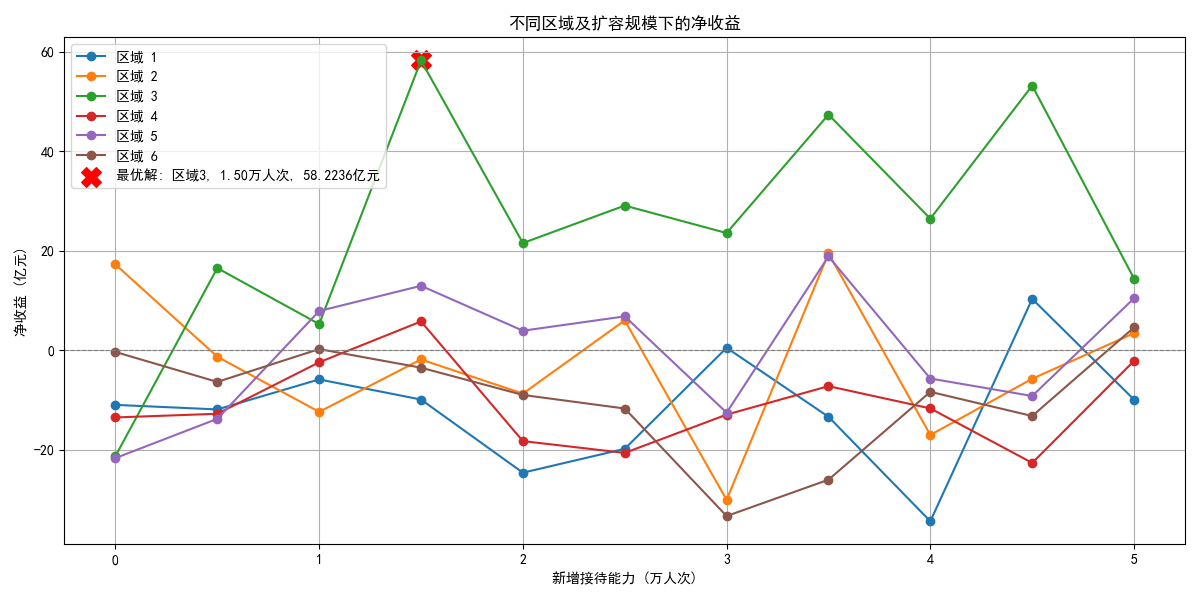
\includegraphics[width=0.8\textwidth]{figures/net_benefit_vs_expansion.png}
  \caption{不同区域扩容规模与净收益关系图}
  \label{fig:net-benefit-expansion}
\end{figure}



